\documentclass{article}

\usepackage{amsmath, amsthm, amssymb}
\usepackage{graphicx, url}
\usepackage{subfig}

\title{Parallel Image Processing}
\author{Keegan Smith \small $<$smtkee002$>$}

\begin{document}

\maketitle

%% Your report must include:
%%   • an introduction, containing a concise description of the
%%      problem.
%%   • A description of the parallel algorithms for both
%%      OpenMP and MPI, highlighting any similarities and/or
%%      differences, any novel/interesting features and
%%      difficulties encountered. This would include how you
%%      dealt with boundary areas, what mode of
%%      communication you used etc.
%%   • Images showing the sample input and sample output
%%      from your code.
%%   • Details of who did what – i.e. how your group
%%      parallelized the task of doing this tutorial! (and a
%%      comment on how efficient this was)
%%   • Analysis of the scalability of your solution. This would
%%      include speedup analysis and graphs with increasing
%%      numbers of processors and increasing image sizes,
%%      and increasing filter size. You will have to think about
%%      how to present this clearly.
%% • It is important to compare the results for OpenMP and
%%   MPI and comment on any differences: which scales
%%   better and why?
%% • Please note, that as this is probably the first parallel
%%   code that you have written, I do not expect your
%%   implementations to have astounding performance and
%%   scalability. However, I do expect you to be able to
%%   reflect on what the problems are and report the results
%%   clearly. Any odd features in the speedup graph should
%%   be commented on. Code that is scaling badly will not
%%   necessarily mean poor marks, but failure to comment
%%   and explain will!
%% • Note that using tools such as SKaMPI to establish the
%%   latency of a cluster, for both ping-pong and collective
%%   messages, may assist in understanding where the
%%   bottlenecks are.


\section{Introduction}

This paper investigates parallising image filtering using a kernel
filter. Kernel filters can be used to do certain transformations on images
such as blurring, embossing, smoothing, etc. A kernel filter is a 2D matrix
which is applied to an image (which is viewed as a 2D collection of color
intensities). How it is applied will be explained in the implementation
section.

This paper investigates four different methods for parallising a kernel
filter. The first implementation uses OpenMP, which is a compiler extension
for parallising code for shared memory systems. The other 3 implementations
are based on MPI, and test different methods for distributing the image.

\section{Implementation}

Let $F$ be a $N \times M$ matrix where $N$ and $M$ are odd numbers. $F$ is our
kernel filter. Let $I$ be a $W \times H$ matrix of grayscale values. A
grayscale value is a number between 0 and 255. $I$ is our image.

Applying $F$ to $I$ we get $I'$ with the following algorithm:

\begin{verbatim}
for h in 1..H:
  for w in 1..W:
    val = 0.0
    for r in 1..M:
      for c in 1..N:
        x = w + c - N / 2
        y = h + r - M / 2
        if (x,y) in I:
          val += (I[y][x] * F[r][c])
    I'[h][w] = round(val)
\end{verbatim}

Note that we need $I$ to be grayscale. This algorithm can be used on an RGB
image by applying it to each colour component.

This algorithm assumes 2D arrays are indexed such that rows are in contiguous
memory locations. This assumption is used for good cache consistency.

This algorithm deals with out of bound values as zero, which is not what is
usually used. But for the purpose of testing parallisation, other forms of
boundary filling do not affect the results.


\subsection{OpenMP Implementation}

This algorithm is nearly embarrassingly parallisable. One simply adds
\begin{verbatim}
#pragma omp parallel for
\end{verbatim}
above the first for loop (for h in 1..H).

$I'_{h,w}$ is written to once for each $(h,w)$, and since each $h$ is assigned
only one process we have no loop dependences. We also have no synchronisation
issues.


\subsection{MPI Implementations}

There are three implementations using MPI. Each implementation uses a
different method to distribute the image and workload. Each implementation
provides two functions, \emph{send\_jobs} and
\emph{get\_job}. \emph{send\_jobs} is run by the master process and each slave
runs \emph{get\_job}. A job represents a task for a process. It is the
following struct:
\begin{verbatim}
typedef struct {
  unsigned char ** image;
  int width, height;

  // Box to work on in image
  int x1, y1, x2, y2;

  int orig_x1, orig_y1;
} job_t;
\end{verbatim}
orig\_x1 and orig\_y1 are the locations of x1 and y1 in the original
image. (image may just be a portion of the image). Each process filters the
region (x1, y1, x2, y2) and sends back the filtered region to the master
process to reconstruct the final image.

Each implementation divides the work up on a row-by-row basis. This was chosen
over a squares to reduce the number of ghost cells to communicate with from 8
to 2.

\paragraph{basic} The master broadcasts the whole image to every
process. Then each process works out from its rank which rows are assigned to
it.

\paragraph{neigh} The master sends to each process what exactly it needs to
filter the image. It does this by looping over each process and doing a
blocking-send. Note that every process is idle at first, so doing a
non-blocking send is not worthwhile since every process will be waiting for
the send. Also note that the messages are large, so latency hiding does not
make a noticeable difference.

\paragraph{ghost} The master process sends what each process owns. Then each
process directly requests from its neighbours for the missing parts of the
image. This is also done with a blocking-send and receive. It is done in a
specific order to prevent deadlocks.


\section{Experimental Setup}

Testing was done on three different setups. Two of the setups where used for
testing OpenMP, while the last one was for testing MPI. Detailed is the most
relevant aspects of the setups which effect the speed. This is computational
speed as well as data transfer speeds.

\paragraph{Intel Core2 Quad Q9400 (fallen)}
This is the machine development was done on. It contains four cores, each
running at 2.66 GHz. It has 4 Gb of DDR2-800 RAM and a 7200rpm SATA hard
drive. The OS is Ubuntu 9.04 Desktop Edition.

\paragraph{Intel Xeon (nightmare)}
The specific machine is nightmare.cs.uct.ac.za. It has 8 cores, each running
at 2.50 GHz. It has 10 Gb of RAM with a network mounted drive. The OS is
Ubuntu 8.04 server edition.

\paragraph{Amazon EC2 (aws)}
These machines where used for testing MPI. The MPI implementation was
OpenMPI. The instances used where \emph{High-CPU Medium Instance}. These
contain 1.7 GB of memory and can sustain transfers between each other at
50MB/s. The processor is an Intel Xeon with 2 cores at 2.33 GHz. Further
information is available at \url{http://aws.amazon.com/ec2/instance-types/}

\section{Results}

Figure \ref{fig:blur} is an example of a blur on a non-random image. Testing
was done on random images with random filters. An example is figure
\ref{fig:random}. The treating of out-of-bounds values as zero can be seen by
the artifacts at the borders.

\begin{figure}
  \centering
  \subfloat[Input]{
    
\includegraphics[width=0.5\textwidth]{images/dog}
  }
  \subfloat[Output]{
    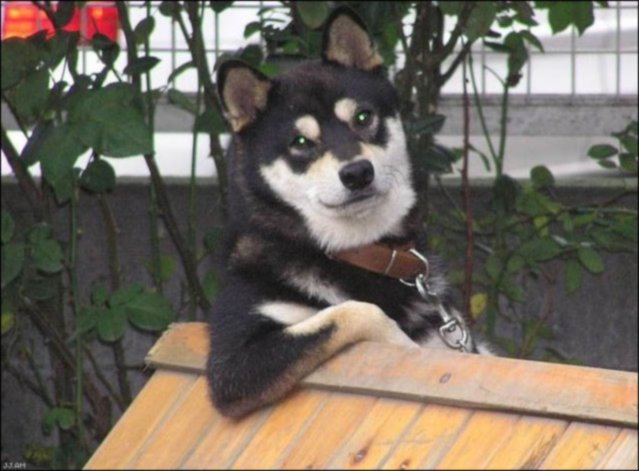
\includegraphics[width=0.5\textwidth]{images/dog_blur}
  }
  \caption{An example run of the OpenMP implementation. The filter used was a 7x7
    gaussian blur.}
  \label{fig:blur}
\end{figure}

\begin{figure}
  \centering
  \subfloat[Input]{
    
\includegraphics[width=0.5\textwidth]{images/random}
  }
  \subfloat[Output]{
    
\includegraphics[width=0.5\textwidth]{images/random_filtered}
  }
  \caption{An example run of the MPI implementation. The input image and the
    filter used where random.}
  \label{fig:random}
\end{figure}

\subsection{OpenMP}

%% \begin{figure}
%%   \centering
%%   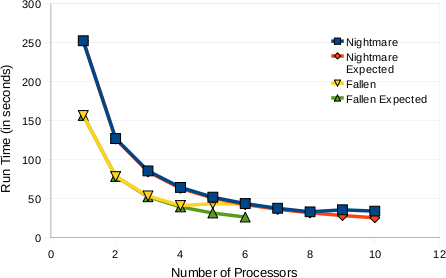
\includegraphics{images/openmp_2000_51}
%%   \caption{OpenMP runs on fallen (4-cores) and nightmare (8-cores). Image was
%%     2000x2000 and filter was 51x51. Expected is the expected run time based on
%%     time taken on 1 core.}
%%   \label{fig:openmp}
%% \end{figure}

Figure \ref{fig:mpi} graphs the run time for the different MPI
implementations. Note that the filter is large so the computation dominates
the runtime. So the differences in speed between different implementations is
not noticeable since communication comprises a minuscule amount of time. A
good indicator is that the expected time is roughly the same as the actual
runtime in all implementations.

\begin{figure}[h]
  \centering
  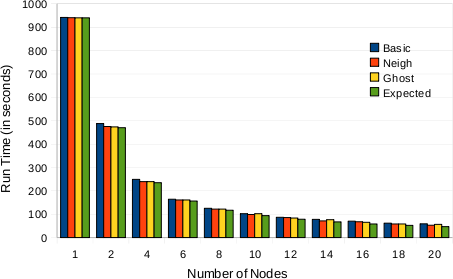
\includegraphics{images/mpi}
  \caption{Run times of different MPI implementations on EC2 with a large
    filter. Image was 5000x5000 and filter was 51x51. Expected is the expected
    run time based on time taken on 1 core for ghost.}
  \label{fig:mpi}
\end{figure}

Figure \ref{fig:mpivsopenmp} gives a more fair representation of the
efficiency of the different communication methods. This is because it uses a
small filter, causing the computation to play a small part of the
runtime. Here it is clear that the neighbour implementation causes the least
amount of communication overhead.

Figure \ref{fig:mpivsopenmp} also includes the OpenMP runtime. It is surprising
to see that the OpenMP implementation is slower in some regards, even though
it has no communication between threads. This may be due to the difference in
disk I/O speeds between EC2 and the Fallen machine.

\begin{figure}[h]
  \centering
  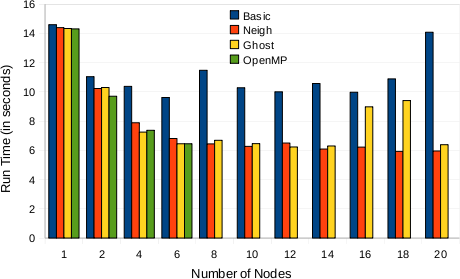
\includegraphics{images/mpi_vs_openmp}
  \caption{Run times of different MPI implementations on EC2 with a small
    filter. Image was 5000x5000 and filter was 5x5. OpenMP run time on fallen
    (4-core) is included for comparison.}
  \label{fig:mpivsopenmp}
\end{figure}

The speedup graph (figure \ref{fig:speedup}) indicates that the algorithms
parallise extremely well. The anomalies in ghost and basic can be attributed
to the fact that this was run in a shared environment, and other users may be
using the network device.

The dip at the end for the OpenMP implementations is due to the number of
processors being used is more than the number of cores. The OpenMP
implementations also have a better speedup than the MPI implementations. It is
suspected that this difference would become more apparent as the number of
cores increase.

\begin{figure}[h]
  \centering
  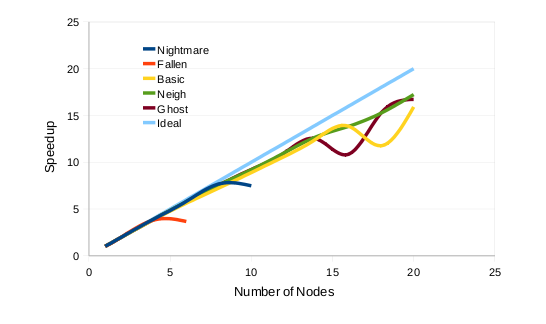
\includegraphics{images/speedup}
  \caption{Speedup graph on 2000x2000 image and 51x51 filter.}
  \label{fig:speedup}
\end{figure}

The size of the filter plays a large part in the runtime. This can be seen in
figure \ref{fig:filter}. This graph is not suprising since the runtime
complexity of the algorithm is $O(|I| \times |F|)$. So we expect a filter of
size $51 \times 51$ to be take four times as long as a filter of size $25
\times 25$.

\begin{figure}[h]
  \centering
  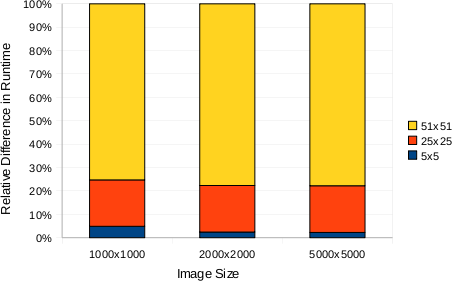
\includegraphics{images/filter}
  \caption{Relative difference in runtime for different filter sizes vs image size.}
  \label{fig:filter}
\end{figure}

\section{Conclusion}

The algorithm parallises extremely well. The OpenMP implementation was simple,
as it was only adding one line to the serial version. The MPI version was more
complex to code, but it has the advantage of being able to scale better than
the OpenMP version. This is because the OpenMP requires a shared memory
machine, while the MPI version works across clusters.

\end{document}
